\documentclass[14pt]{extarticle}
\usepackage{fontspec}
\usepackage{polyglossia}
\usepackage{amsmath}
\usepackage{amssymb}
\usepackage{xcolor}
\usepackage{fancyhdr}
\usepackage{graphicx}
\usepackage{listings}
\usepackage[most]{tcolorbox}
% \usepackage{setspace}
\usepackage{pifont}
\usepackage{enumitem}
\usepackage{titlesec}
\usepackage[bottom]{footmisc}
\usepackage{titling}
\usepackage{minted}
\usepackage{etoolbox}
\usepackage{array}
\usepackage{extsizes}
\usepackage{float}
\usepackage{booktabs}
\usepackage{hyperref}
\usepackage[onehalfspacing]{setspace}
\usepackage[a4paper, top=2.7cm, bottom=2.7cm, left=2.5cm, right=2.5cm, headheight=1.5cm, headsep=0.5cm]{geometry}
\usepackage{tikz}

\usetikzlibrary{automata, positioning, arrows.meta, arrows}

\newfontfamily\emoji{Segoe UI Emoji}

\pagestyle{fancy}

\setmainlanguage[numerals=western]{arabic}
\setotherlanguage{english}
% \newfontfamily\arabicfont[Script=Arabic]{Amiri}
\newfontfamily\arabicfont[Script=Arabic]{Calibri}
\newfontfamily\arabicfonttt[Script=Arabic]{Courier New}

\lstset{
  language=[Sharp]C,
  numbers=left,
  stepnumber=1,
  numbersep=8pt,
  frame=single,
  basicstyle=\ttfamily\small,
  keywordstyle=\color{blue},
  stringstyle=\color{red},
  commentstyle=\color{green!50!black}
}

\newif\ifdetailed
\ifdefined\setdetailed
  \setdetailed
\fi

\newif\ifwithsols
\ifdefined\setwithsols
  \setwithsols
\fi

% unified tcolorboxes for articles
\tcbset{colback=white, colframe=black, fonttitle=\bfseries, boxrule=0.8pt}
\newtcolorbox{boxDef}[1][]{colback=blue!5!white,colframe=blue!75!black,
  title={{\emoji📘} تعريف\ifx\\#1\\\else ~#1\fi :}}
\newtcolorbox{boxExercise}[1][]{colback=cyan!5!white,colframe=cyan!70!black,
  title={{\emoji🧩} تمرين\ifx\\#1\\\else ~#1\fi :}}
\newtcolorbox{boxExample}[1][]{colback=yellow!5!white,colframe=orange!90!black,
  title={{\emoji📝} مثال\ifx\\#1\\\else ~#1\fi :}}
\newtcolorbox{boxNote}[1][]{colback=gray!10!white,colframe=black,
  title={{\emoji✨} ملاحظة\ifx\\#1\\\else ~#1\fi :}}
\newtcolorbox{boxAttention}[1][]{colback=magenta!10!white,colframe=magenta!80!black,
  title={{\emoji🔔} تنبيه\ifx\\#1\\\else ~#1\fi :}}
\newtcolorbox{boxWarning}[1][]{colback=red!5!white,colframe=red!75!black,
  title={{\emoji⚡} ملاحظة هامة\ifx\\#1\\\else ~#1\fi :}}
\newtcolorbox{boxSolution}[1][]{colback=green!5!white,colframe=green!60!black,
  title={{\emoji✅} حل\ifx\\#1\\\else ~#1\fi :}}
\newtcolorbox{boxSymbol}[1][]{colback=purple!5!white,colframe=purple!70!black,
  title={{\emoji🔣} رمز\ifx\\#1\\\else ~#1\fi :}}
\newtcolorbox{boxHint}[1][]{colback=teal!5!white,colframe=teal!60!black,
  title={{\emoji💡} تلميح\ifx\\#1\\\else ~#1\fi :}}


\tcbset{simplecode/.style={ colback=gray!5, colframe=black!50, boxrule=0.4pt, arc=2pt, left=4pt,right=4pt,top=4pt,bottom=4pt}}
\newenvironment{boxCode}{\begin{tcolorbox}[simplecode]}{\end{tcolorbox}}

\newcolumntype{C}[1]{>{\centering\arraybackslash}p{#1}}

% redefine spaces after titles
\makeatletter
\renewcommand{\@maketitle}{%
  \begin{center}
    {\huge \bfseries \@title \par}%
    \vskip 0.2em % space between title and author
    {\large \@author \par}%
    % \vskip 0.2em % space between author and date
    % {\normalsize \@date \par}%
  \end{center}
}
\makeatother

\fancyhf{} % clear default
\fancypagestyle{plain}{
  \fancyhf{}
  \fancyhead[L]{مدرسة التسامح الشاملة}
  % \fancyhead[L]{
\includegraphics[height=1cm]{../../../images/logoTasamoh.png}}
  \fancyhead[R]{الأستاذ محمود اغبارية}
  \fancyfoot[C]{\thepage}
}

\fancyhead[L]{مدرسة التسامح الشاملة}
\fancyhead[R]{الأستاذ محمود اغبارية}
\fancyfoot[C]{\thepage}
% \date{\today}

\setcounter{tocdepth}{3} % only section subsection and subsubsection in TOC

\newcommand{\importpdfpage}[2]{%
    \thispagestyle{empty}
    \newgeometry{left=0cm,right=0cm,top=0cm,bottom=0cm}
    \includegraphics[page=#2,width=0.95\paperwidth,height=0.95\paperheight,keepaspectratio]{#1}
    \restoregeometry
}

\newcommand{\insertFullImg}[1]{%
    \noindent
    \makebox[\textwidth][c]{
        \includegraphics[width=0.9\paperwidth,keepaspectratio]{#1}%
    }%
}%

% ----------------------


% \begin{document}

% \maketitle

% % \clearpage  % start TOC on a new page
% % \renewcommand{\contentsname}{جدول المحتويات}
% % \tableofcontents
% % \clearpage

% \part*{part 1} % the * prevents numbering
% \section*{مقدمة}
% \subsection*{مثال رياضي}
% \subsubsection*{مثال فرعي}
% \paragraph*{ paragraph 1}
% \subparagraph*{sub paragraph 1}

% \ifdetailed
% \begin{english}
% \begin{minted}{csharp}
% // C# Example
% \end{minted}
% \end{english}
% \fi

% OLD WAY
% \ifdetailed
% \begin{english}
% \begin{lstlisting}
% // C# Example
% \end{lstlisting}
% \end{english}
% \fi

% % 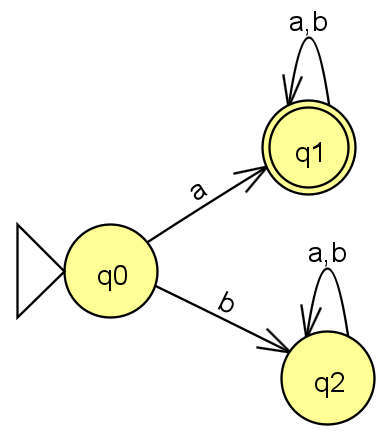
\includegraphics[width=0.2\textwidth]{../../../images/DFAs/ex1_q1.png}



% \vspace{3cm}
% \begin{flushleft}
% أرجو لكم وقتًا ممتعًا.

% الأستاذ محمود اغبارية.
% \end{flushleft}


% \end{document}


\ifwithsols
\title{حل وظيفة 10: آلة تورينج}
\else
\title{وظيفة 10: آلة تورينج}
\fi

\begin{document}

\maketitle

% \begin{enumerate}[itemsep=2em]
% \item صمّم آلة تيورنج تتلقى عددَين أوناريّين $x$ و$y$ مفصولين بإشارة $\#$،  وتحسب الدالة:
% \[f(x,y) = \max(x,y)\]
% وتكتب النتيجة بالتمثيل الأوناري بين إشارتَي $\$$ في مكانٍ ما على الشريط. \\
% \textbf{مثال}

% \textbf{المدخل ($x=5$, $y=3$):} \\
% \begin{tikzpicture}[scale=0.85]
%     \foreach \i/\c in {1/$\vdash$,2/1,3/1,4/1,5/1,6/$\#$,7/1,8/1,9/1,10/$\triangle$} {
%         \draw (\i,0) rectangle +(1,0.8);
%         \node at (\i+0.5,0.4) {\c};
%     }
% \end{tikzpicture}

% \vspace{0.5em}

% \textbf{الناتج ($\max(5,3)=5$):} \\
% \hspace{0.5em}
% \begin{tikzpicture}[scale=0.85]
%     \foreach \i/\c in {1/$\vdash$,2/$\ldots$,3/$\$$,4/1,5/1,6/1,7/1,8/1,9/$\$$,10/$\ldots$} {
%         \draw (\i,0) rectangle +(1,0.8);
%         \node at (\i+0.5,0.4) {\c};
%     }
% \end{tikzpicture}

% \ifwithsols
% \begin{boxSolution}
% \begin{center}
%     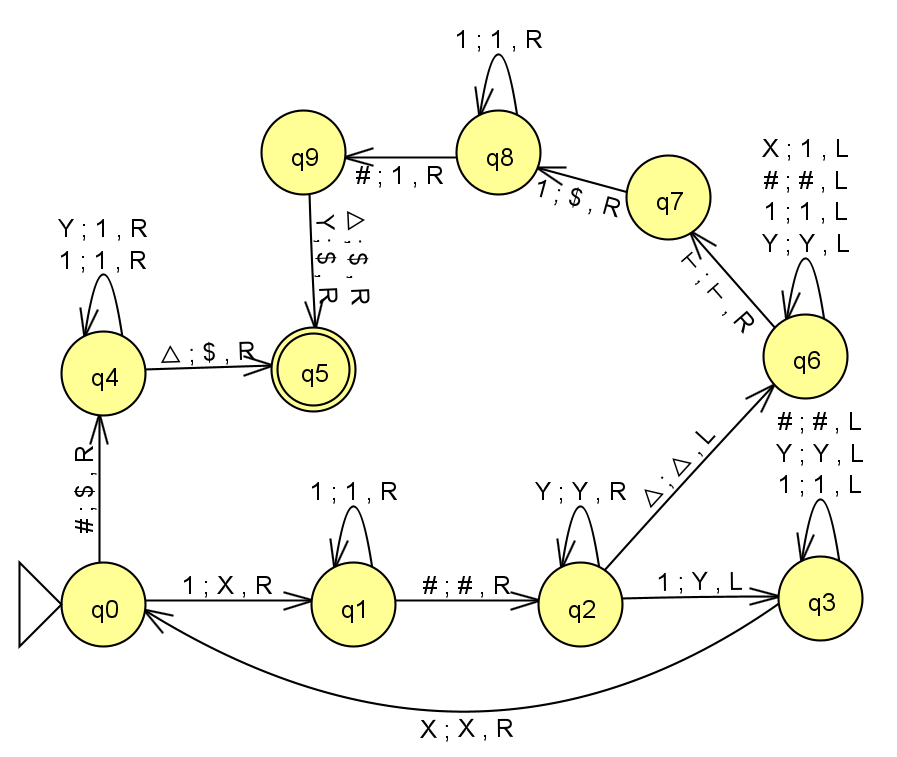
\includegraphics[width=0.4\paperwidth,keepaspectratio]{../../../images/turing/fx_max_xy.png}%
% \end{center}
% \end{boxSolution}
% \fi

% \end{enumerate}

\subsection*{سؤال 12 امتحان 899381 سنة 2019}
\addcontentsline{toc}{subsection}{سؤال 12 امتحان 899381 سنة 2019}

\noindent
\makebox[\textwidth][c]{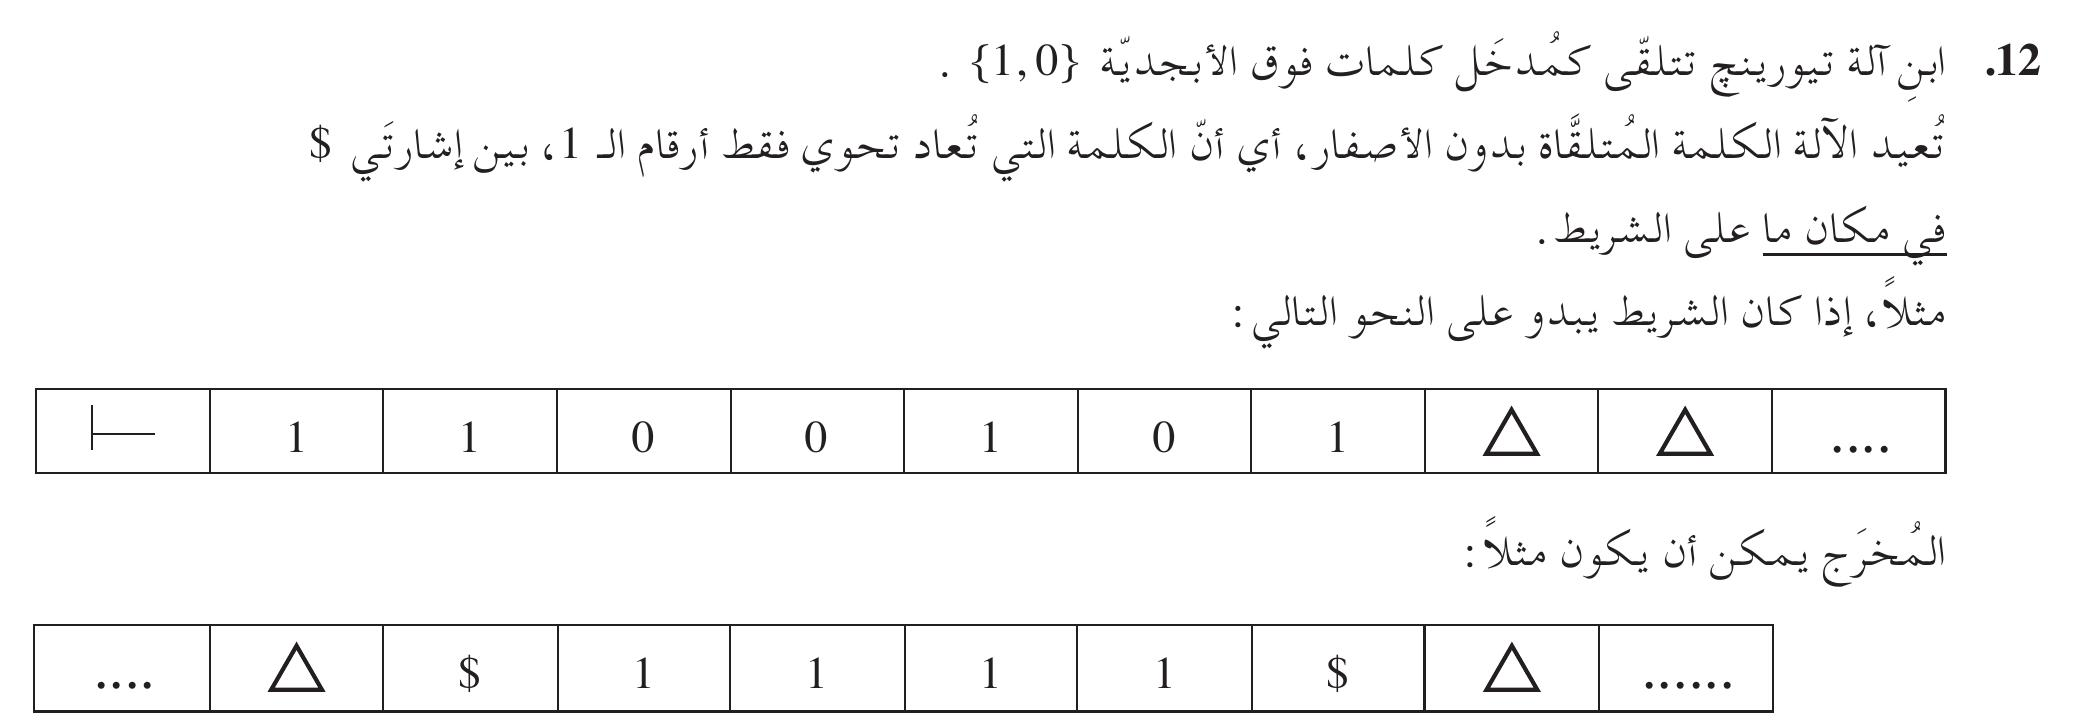
\includegraphics[width=0.9\paperwidth,keepaspectratio]{ ../../../bagrut_questions/computational_models/turing_2019_899381_12.jpg }%
}%

\ifwithsols
\begin{boxSolution}[سؤال 12 امتحان 899381 سنة 2019]
\begin{center}
    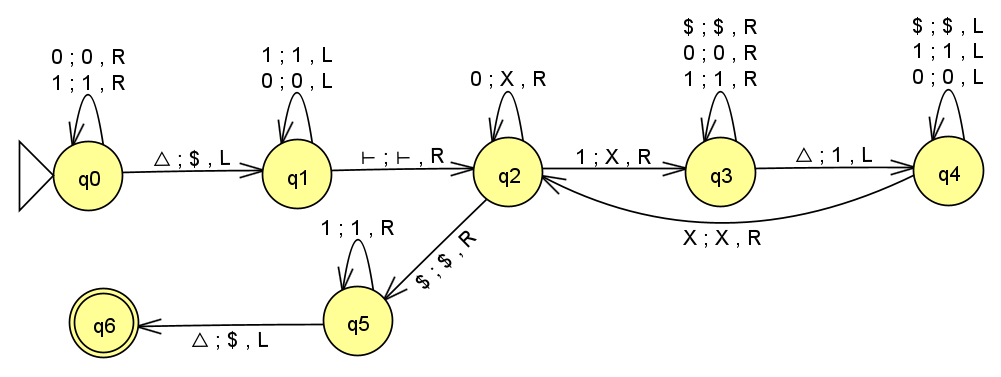
\includegraphics[width=0.7\paperwidth,keepaspectratio]{../../../images/turing/cancel_zeros_keep_ones.png}%
\end{center}

\end{boxSolution}

\fi


\subsection*{سؤال 13 امتحان 899205 سنة 2014}
\addcontentsline{toc}{subsection}{سؤال 13 امتحان 899205 سنة 2014}

\noindent
\makebox[\textwidth][c]{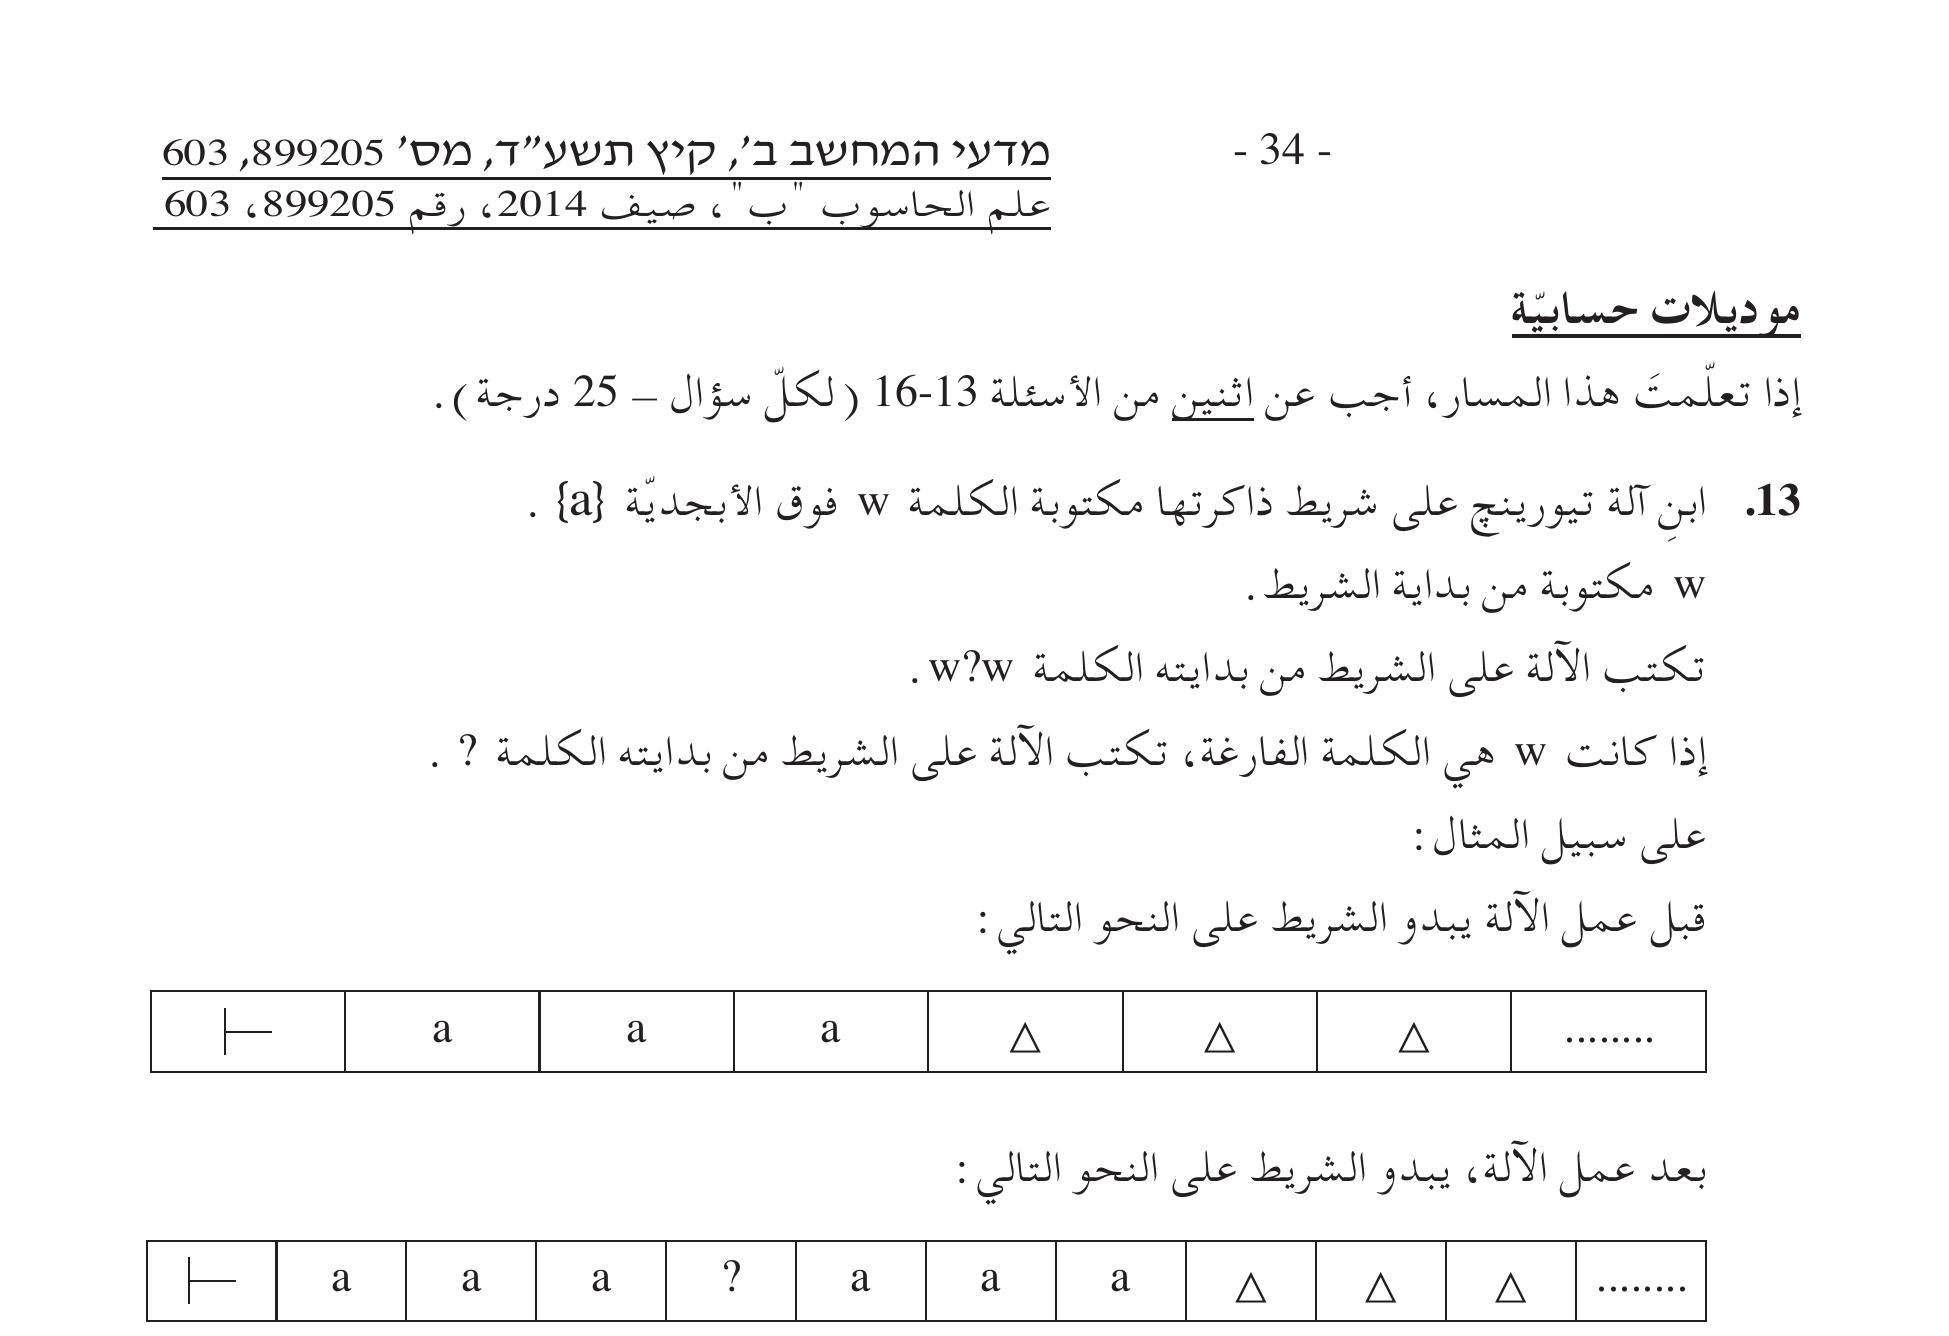
\includegraphics[width=0.9\paperwidth,keepaspectratio]{ ../../../bagrut_questions/computational_models/Turing_2014_899205_13.jpg }%
}%

\ifwithsols
\begin{boxSolution}[سؤال 13 امتحان 899205 سنة 2014]
\begin{enumerate}[itemsep=1.5em, label=\alph*.]
    \item // TODO:
\end{enumerate}
\end{boxSolution}

\fi

\ifwithsols
\else
\clearpage
\fi

\subsection*{سؤال 12 امتحان 899381b سنة 2016}
\addcontentsline{toc}{subsection}{سؤال 12 امتحان 899381b سنة 2016}

\noindent
\makebox[\textwidth][c]{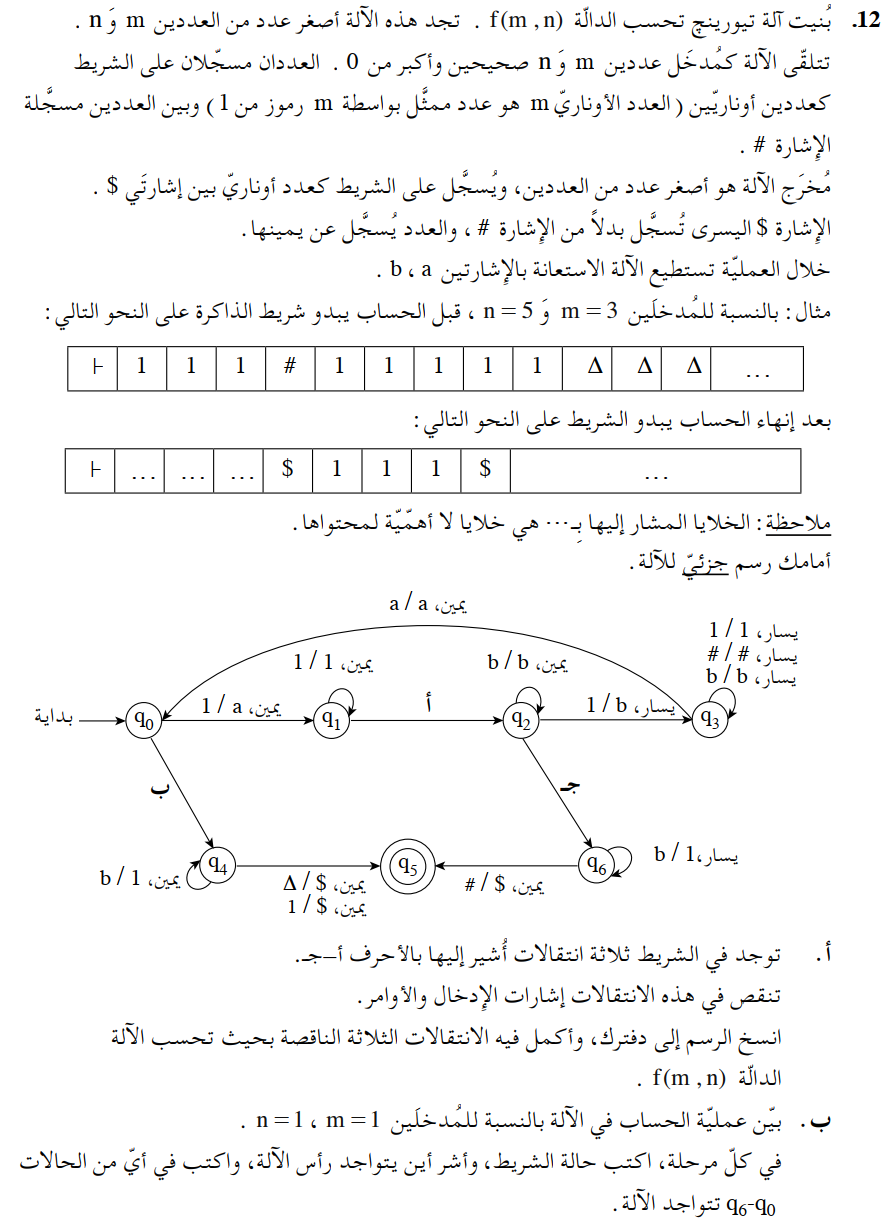
\includegraphics[width=0.75\paperwidth,keepaspectratio]{ ../../../bagrut_questions/computational_models/Turing_2016_899381b_12.png }%
}%

\ifwithsols
\begin{boxSolution}[سؤال 12 امتحان 899381b سنة 2016]
\begin{enumerate}[itemsep=1.5em, label=\alph*.]
    \item // TODO:
\end{enumerate}
\end{boxSolution}

\clearpage
\fi


\end{document}
